% SIAM Shared Information Template
% This is information that is shared between the main document and any
% supplement. If no supplement is required, then this information can
% be included directly in the main document.

%In this section we study the impact of parameter $\epsilon_s$ and hardware parallelism on the quality of  \acrshort{RACE} method. \Inorder to do this we first quantify the quality of the method and finally we  use this quantity to do a parameter study. The study gives insights into tuning of parameter $\epsilon_s$ based on the given matrix and required parallelism.


The \acrshort{RACE} method has a set of input
parameters $\{\epsilon_s; s=0,1,\ldots\}$ which control the
assignment of threads to adjacent level groups.
%For that reason a good choice is to have values close to $1$ for the initial stages and have a more relaxed constraint on the lower levels. 
To determine useful settings, we analyze the interaction
between these input parameters, the number of threads used, and the
parallel efficiency of the generated workload distribution.

As the internal tree structure contains all information about the
final workload distribution, we can use it to identify the critical
path in terms of workload and thus \rAdd{identify} the parallel
efficiency. To this end we introduce the \effRow for every node
(or \levelGroup) $\acrshort{nrowsEff}(T_s(i))$, which is a measure for
the absolute runtime to calculate the
corresponding \levelGroup. For \levelGroups that are not further
refined (\rAdd{\ie the} leaf nodes) this value is their actual workload, \ie the
number of rows assigned to them ($\acrshort{nrowsEff}(T_0(0)) = 15$
in \Cref{fig:rec_2d-7pt_tree}). For an inner node, the \effRow is the
sum of the maximum workload (\ie the maximum \effRow value) across each of
the two colors of its child nodes:
\begin{align*}
\acrshort{nrowsEff}(T_s(i)) &= \max\left(\acrshort{nrowsEff}(T_{s+1}(j) \subseteq T_s(i))\right) + \max\left(\acrshort{nrowsEff}(T_{s+1}(j+1) \subseteq T_s(i))\right)\\
 & \text{for } j=0,2,\ldots
\end{align*}
Such a definition is based on the idea that nodes at a given stage $s$
have to synchronize with each other and have to wait for their
siblings with the largest workload in each \rDel{sweep (color)} \rAdd{color}. Propagating
this information upwards on the tree until we reach the root node
constructs the critical path in terms of longest runtime taking into
account single thread workloads, dependencies, and
synchronizations. Thus, the final value in the root node
$\acrshort{nrowsEff}(T_{-1}(0))$ can be considered as the effective
maximum workload of a single thread. Dividing the globally optimal
workload per thread,
${\acrshort{nrows}^\mathrm{total}}/{\acrshort{nthreads}}$, by
this number gives the parallel efficiency ($\eta$) of our workload
distribution:
\begin{align*}
	\eta &= \frac{ \acrshort{nrows}^\mathrm{total}} {\acrshort{nrowsEff}(T_{-1}(0)) \times \acrshort{nthreads}}. 
\end{align*}
For the tree presented in \Cref{fig:rec_2d-7pt_tree}, the parallel
efficiency is limited to $\eta=\frac{256}{44 \times 8 } = 0.73$ on
eight threads, \ie the maximum parallel speedup is $5.8$.

\subsection{Parameter analysis and selection}
\label{subsec:param_analysis}
The parallel efficiency \acrshort{eta} as defined above can be calculated for
any given matrix, number of threads $\acrshort{nthreads}$, and choice of
$\{\epsilon_s; s=0,1,\ldots\}$; it reflects the quality of parallelism generated
by \acrshort{RACE} for the problem at hand.  This way we can understand the
interaction between these parameters and identify useful choices for
the $\epsilon_s$. Of course, running a specific kernel such
as \acrshort{SymmSpMV} on actual hardware will add further hardware and software
constraints such as attainable memory bandwidth or cost of synchronization.

As a first step we can limit the parameter space by simple corner case
analysis. 
\rAdd{The lowest possible value of $\epsilon_s$ is the 
	maximum deviation of a real number from
	its nearest integer, which is $0.5$. On the other
hand the highest possible value is one.}
Setting all parameters ($\epsilon_s$) close to one requests high-quality load
balancing but may prevent our balancing scheme from terminating. 
In the extreme
case of $\{\epsilon_s=1; s=0,1,\ldots\}$ the scheme may generate only
two \levelGroups (one of each color) in each recursion, assign all threads to
them, and may further attempt to refine them in the same way.  
\rDel{The lowest possible value of $\epsilon_s$ is the 
	maximum deviation of a real number from
its nearest integer, which is $0.5$.}
 A range of [$0.5$,$0.9$] for the
$\epsilon_s$ is therefore used in the following \rAdd{analysis}. 
\rAdd{To ensure termination the default $\epsilon_s$ value is 
	chosen to be 0.5. Due to this even if sufficient parallelism cannot
	be found at a user specified $\epsilon_s$ value for lower 
	recursive stages the algorithm can move to higher stages
	(with default $\epsilon_s = 0.5$) and terminate.}	
%	 which allows the algorithm to 
%	terminate at a higher recursive stage even if a high $\epsilon_s$ 
%	value is specified at lower stages.}

For \rDel{a basic analysis}
\rAdd{an initial discussion} we have
selected the \emph{inline\_1} matrix (see \Cref{tab:test_mtx}), \rAdd{which has a
rather small amount of parallelism and thus represents an important
corner case}. In \Cref{fig:inline_param_study} we demonstrate the impact of
different choices for $\epsilon_0$ and $\epsilon_1$ on the parallel efficiency
for thread counts up to 100, which is a useful limit for modern CPU-based
compute nodes.
%
\begin{figure}[t]
	\centering
	\subfloat[$\eta$ versus \acrshort{nthreads} for \emph{inline\_1} matrix, $\epsilon_1 = 0.5$ ]{\label{fig:inline-a}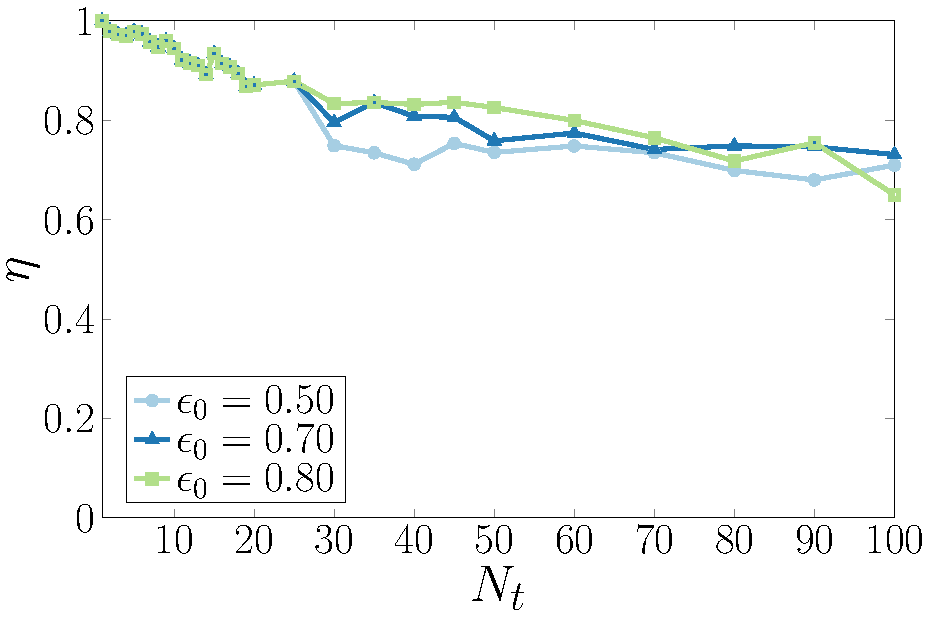
\includegraphics[width=0.45\textwidth , height=0.2\textheight]{pics/param_study/threads_vs_eff}}
	\hspace{1.5em}
	\subfloat[\acrshort{nthreads}=25]{\label{fig:inline-b}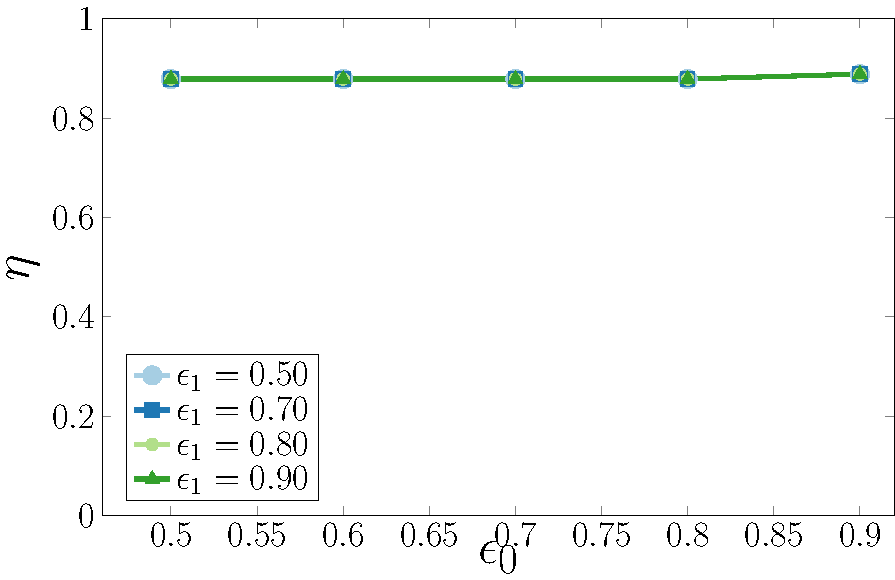
\includegraphics[width=0.45\textwidth , height=0.2\textheight]{pics/param_study/scaling_eps_1_25_threads}}
	
	\subfloat[\acrshort{nthreads}=45 ]{\label{fig:inline-c}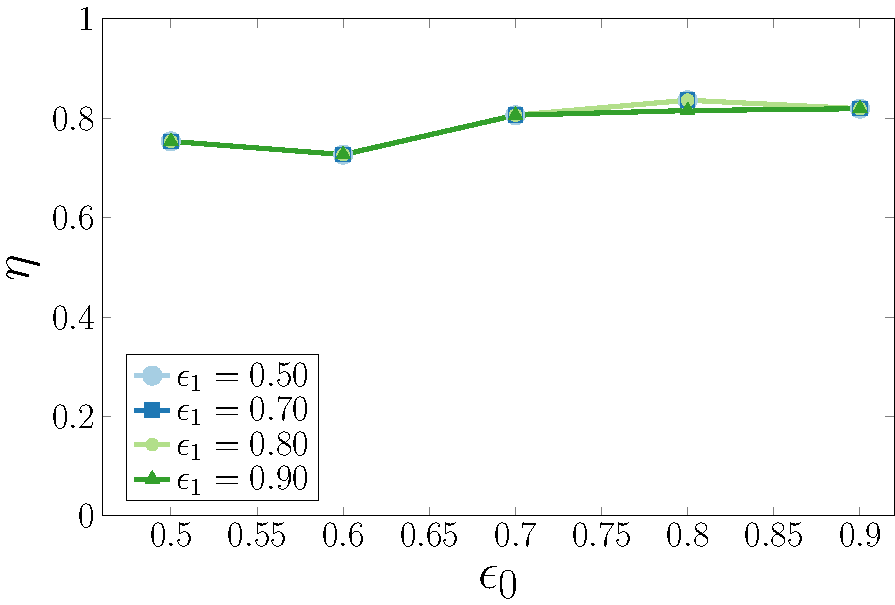
\includegraphics[width=0.45\textwidth , height=0.2\textheight]{pics/param_study/scaling_eps_1_45_threads}}
	\hspace{1.5em}
	\subfloat[\acrshort{nthreads}=100 ]{\label{fig:inline-d}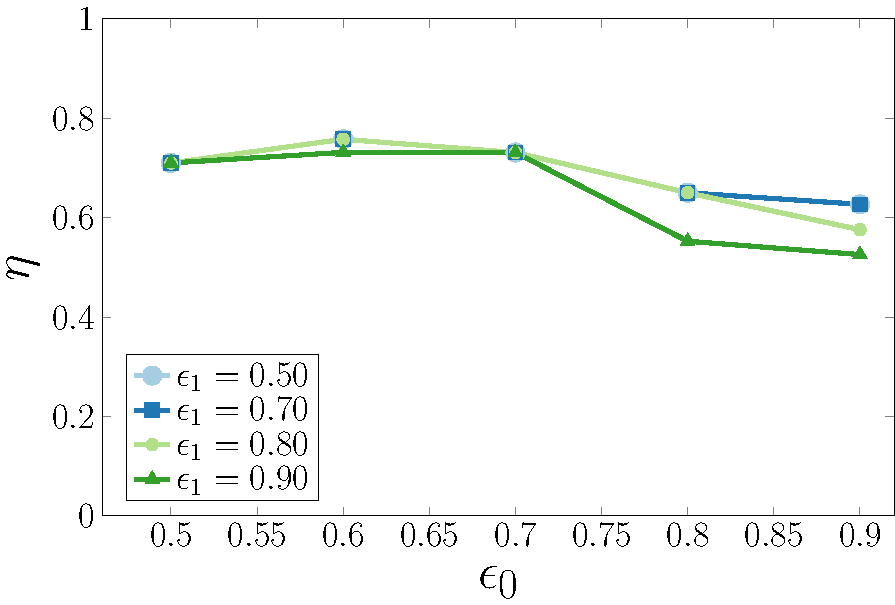
\includegraphics[width=0.45\textwidth , height=0.2\textheight]{pics/param_study/scaling_eps_1_100_threads}}
	\caption{Parameter study on the \emph{inline\_1} matrix. In \Cref{fig:inline-b,fig:inline-c,fig:inline-d} each of the lines in the plot are iso-$\epsilon_1$ and impact of $\eta$ with respect to $\epsilon_0$ is shown. $\epsilon_s$ for $s>1$ is fixed to $0.5$.}
	\label{fig:inline_param_study}
\end{figure}
%
For $s > 1$ we always set the \rDel{minimum} \rAdd{default} value of $\epsilon_s=0.5$. The limited
parallelism can be clearly observed in \Cref{fig:inline-a}, with efficiency
steadily decreasing with increasing thread count. At
$\epsilon_1=0.5$ there is only a minor impact of the parameter
$\epsilon_0$ \rAdd{for small thread counts ($\acrshort{nthreads}<30$)}. In \Cref{fig:inline-b,fig:inline-c,fig:inline-d} the interplay
between these two parameters is analyzed at different thread counts in more
detail. We find that up to intermediate parallelism ($\acrshort{nthreads}=50$)
the exact choice has only a minor impact on the parallel efficiency 
\rDel{(see $y$-axis scaling)}. %\rAdd{(the axis are scaled similarly)}.
For larger parallelism the interplay becomes more intricate,
where too large values of $\epsilon_{0,1}$ may lead to stronger imbalance. Based
on this evaluation, we choose $\epsilon_{0,1}=0.8$ and $\epsilon_s=0.5$ for $s>1$
for all subsequent performance measurements. The quality of this choice in terms of
parallel efficiency for all matrices is presented
in \Cref{fig:param_all_mtx_stat}. Here we plot the $\eta$ value for all the
matrices over a large thread count. We find that our parameter setting achieves
parallel efficiencies \rDel{of 80\% or higher for a substantial fraction of the
matrices up to intermediate thread counts.}
\rAdd{of 75\% or higher for 75\% of the matrices up to an intermediate thread count of 40. }
   \begin{figure}[t]
   	\centering
   	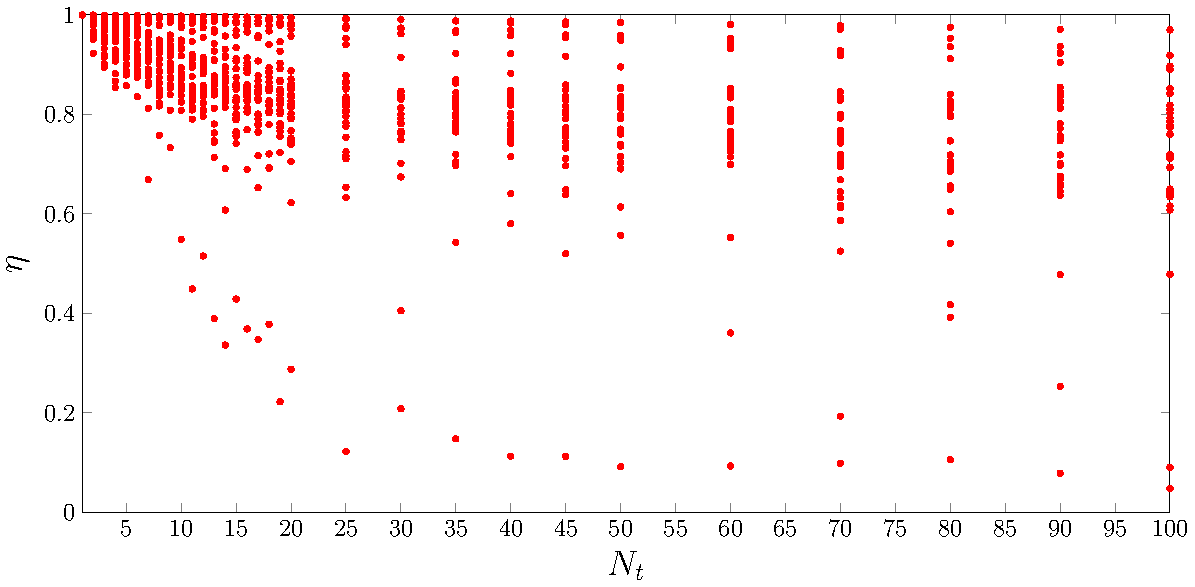
\includegraphics[width=0.9\textwidth]{pics/param_study/scatter_plot}
   	\caption{Parallel efficiency $\eta$ versus \acrshort{nthreads} for all test matrices with $\epsilon_{0,1} = 0.8$ and $\epsilon_{s>1} = 0.5$.}
  	\label{fig:param_all_mtx_stat}
   \end{figure}
Representing the upper (lower) values in \Cref{fig:param_all_mtx_stat} is the
best (worst) case matrix \emph{Graphene-4096} (\emph{crankseg\_1}), exhibiting
almost perfect (very low) parallel efficiency at intermediate to high thread
counts.

Finally, we evaluate the scalability of RACE using these two corner cases and
the \emph{inline\_1} matrix as well as the \emph{parabolic\_fem} matrix.
\rDel{, which} \rAdd{The latter}
is small enough to fit into the cache.  In \Cref{fig:corner_cases_param} we
mimic scaling tests on one Skylake processor with up to 20 cores (\ie
threads) and plot the parallel efficiency $\eta$ as well as the maximum number
of threads which can be ``perfectly'' used \acrshort{threadEff} (\ie
$\acrshort{threadEff} = \eta\times\acrshort{nthreads}$).  The unfavorable structure
of the \emph{crankseg\_1} matrix puts strict limits on parallelism even for low
thread counts.  The combination of small matrix size with a rather dense
population (see \Cref{table:bench_matrices}) leads to large inner levels when
constructing the graph, triggering strong load imbalance \rDel{if} 
\rAdd{when} using more than six threads.
A search for better $\epsilon_s$ slightly changes the \rDel{characteristic}
scaling \rAdd{characteristic} but not the maximum parallelism that can be extracted. 
For the \emph{inline\_1} matrix we find a weak but steady decrease of the parallel
efficiency, which is in good agreement with the discussion
of \Cref{fig:inline_param_study}. The other two matrices scale very well in the
range of thread counts considered.


The corresponding performance measurements for the \acrshort{SymmSpMV} kernel
(see \Cref{sect:SymmSpmv}) on a single \SKX processor chip with 20 cores are
shown in \Cref{fig:corner_cases_scaling}.\footnote{For the benchmarking setup
see \Cref{Sec:expt}.}
%A strong relationship between the theoretical  (\Cref{fig:corner_cases_param}) and  experimental (\Cref{fig:corner_cases_scaling}) scaling graph can be clearly observed. 
For the \emph{crankseg\_1} matrix (see \Cref{fig:crankseg_scaling}) we recover
the limited scaling due to load imbalance as theoretically predicted. A
performance maximum is at nine cores, where the maximum \acrshort{SpMV}
performance can be slightly exceeded. However, based on the \roofline performance
model given by \Cref{eq:SymmSpMV_intensity,eq:upper_performance} together with
the matrix parameters from \Cref{table:bench_matrices}, a theoretical speedup of
approximately two as compared to \acrshort{SpMV} can be expected for the full
processor chip under best conditions.
Indeed, in case of the \emph{inline\_1} and \emph{Graphene-4096}
matrices, performance
scales almost linearly until the main memory bandwidth bottleneck is hit. The
saturated performance is in good agreement with the \roofline limits.
%although the experimental and theoretical results match for the initial phase it shows a different behavior towards the end. This happens since the kernel saturates the memory bandwidth available for this chip, which can be easily verified by observing the close agreement of the full socket performance and the performance model prediction given by \Cref{eq:SymmSpMV_intensity,eq:upper_performance}. 
Note that even though the \emph{inline\_1} matrix does not exhibit
perfect theoretical efficiency ($\eta$ $\approx 0.85$ at
$\acrshort{nthreads}=20$), it still generates sufficient parallelism to achieve
main memory saturation: \rDel{The} \rAdd{the} memory bottleneck can mitigate
a limited load imbalance.

%The only affect of the lower efficiency was a shift in saturation point to further right (at higher thread count) compared to \emph{Graphene-4096}. 
The peculiar performance behavior of
\emph{parabolic\_fem}
(see \Cref{fig:parabolic_fem_param,fig:parabolic_fem_scaling}) is due to 
its smallness ($\approx 23$ \MB), which lets it fit into the caches of the
Skylake processor (\acrshort{LLC} size $= 28$ \MB). Thus, performance is not
limited by the main memory bandwidth constraint and the \roofline model limits do
not apply.
\begin{figure}[t]
	\centering
	\subfloat[\emph{crankseg\_1}]{\label{fig:crankseg_param}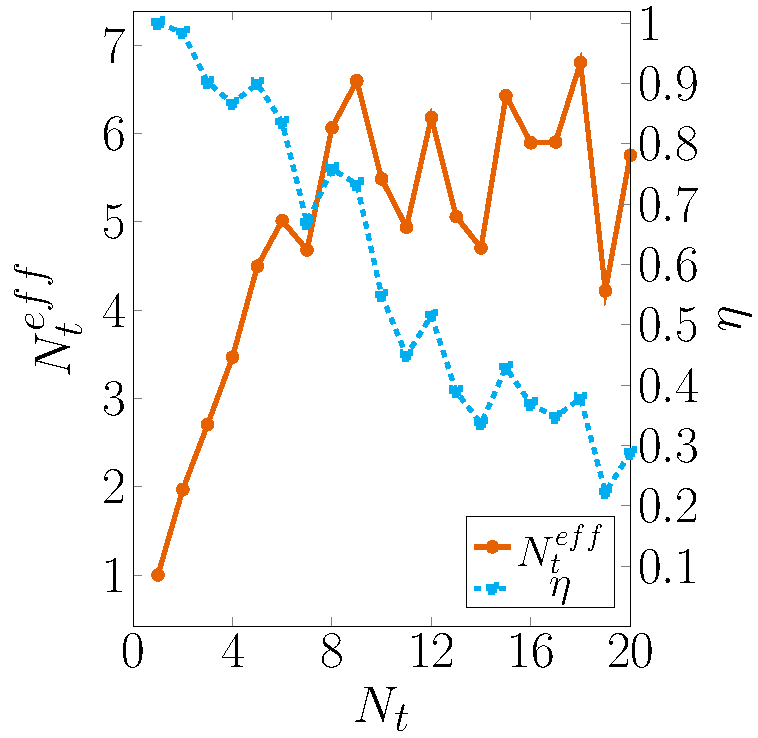
\includegraphics[width=0.24\textwidth]{pics/param_study/corner_cases/crankseg_1}}
	\subfloat[\emph{inline\_1}]{\label{fig:inline_param}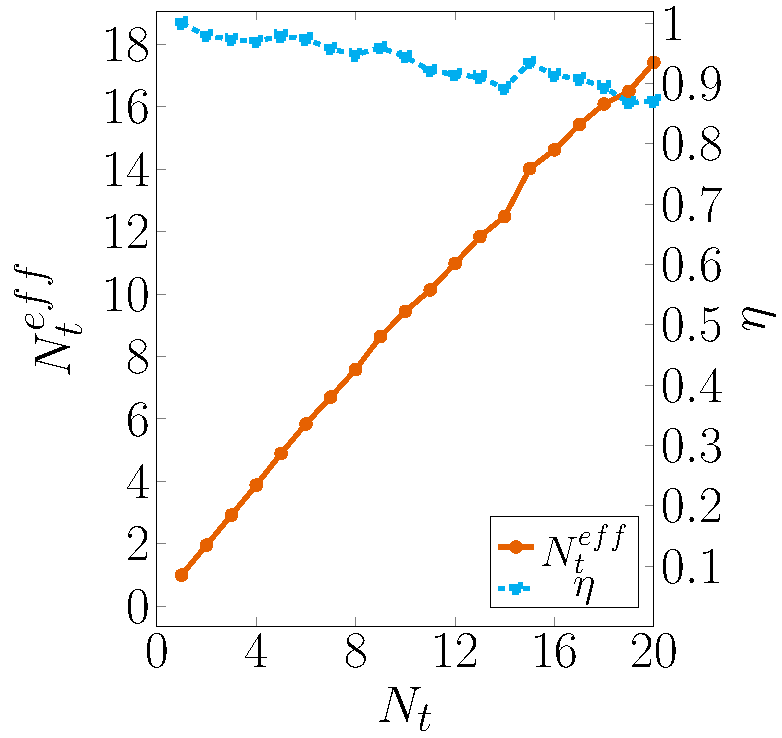
\includegraphics[width=0.24\textwidth]{pics/param_study/corner_cases/inline_1}}	
	\subfloat[\emph{parabolic\_fem}]{\label{fig:parabolic_fem_param}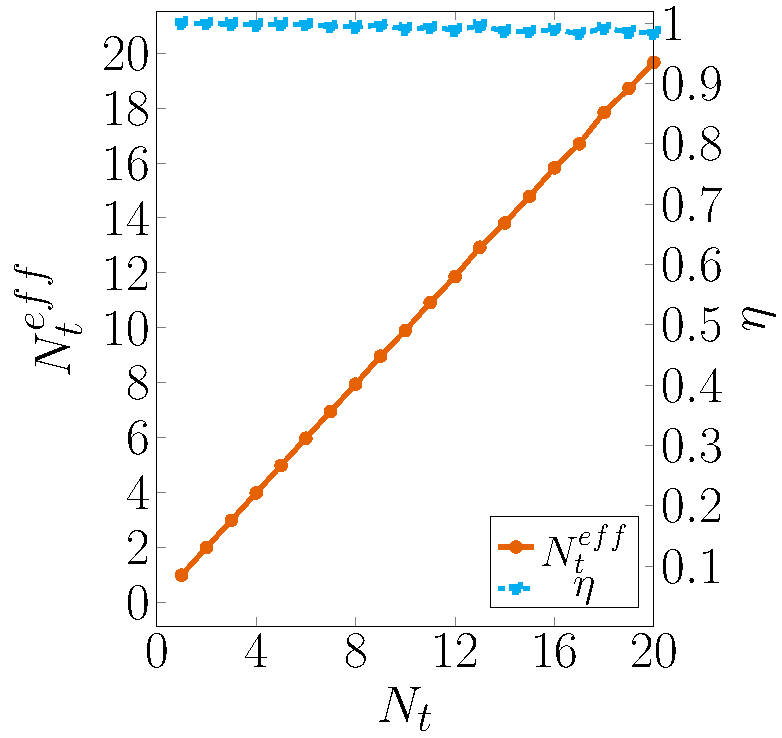
\includegraphics[width=0.24\textwidth]{pics/param_study/corner_cases/parabolic_fem}}
	\subfloat[\emph{Graphene-4096}]{\label{fig:Graphene-4096_param}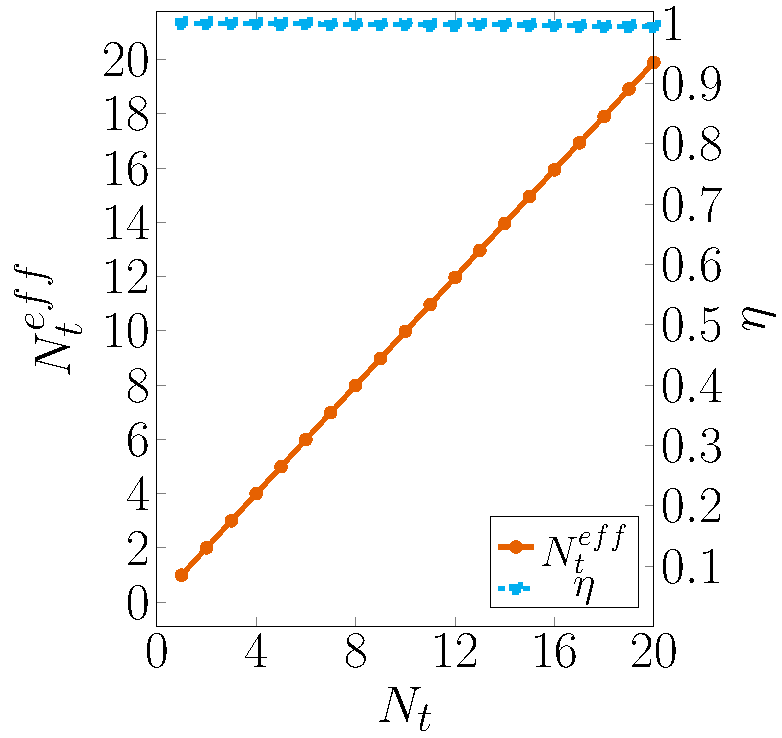
\includegraphics[width=0.24\textwidth]{pics/param_study/corner_cases/Graphene-4096}}	
	\caption{\acrshort{threadEff} and $\eta$ versus \acrshort{nthreads} for
	the four corner case matrices, with the same settings used in experiment
	runs. \acrshort{threadEff} is defined as
	$\eta\times\acrshort{nthreads}$.}
	\label{fig:corner_cases_param}
\end{figure}
\begin{figure}[t]
	\centering
	\subfloat[\emph{crankseg\_1}]{\label{fig:crankseg_scaling}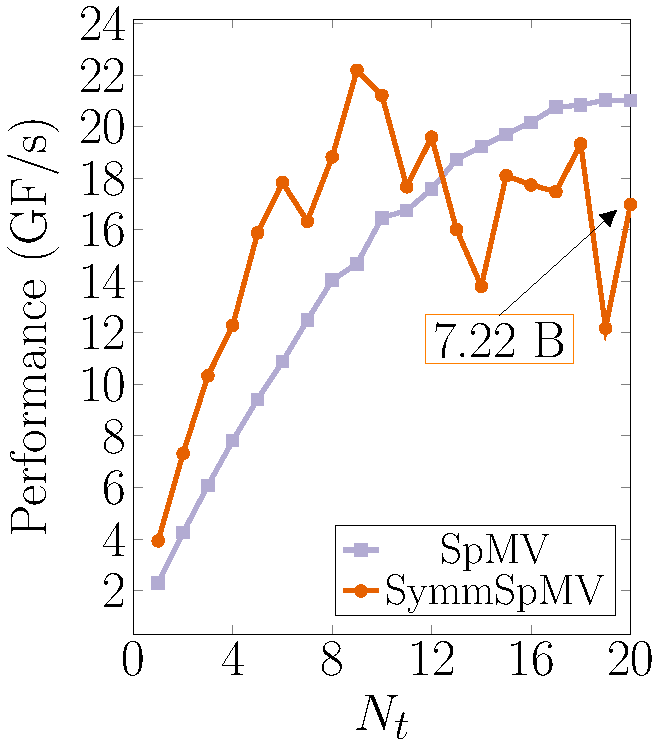
\includegraphics[width=0.23\textwidth , height=0.18\textheight]{pics/results/skx/corner_cases_scaling/plots/RCM/crankseg_1_RCM}}
	\subfloat[\emph{inline\_1}]{\label{fig:inline_scaling}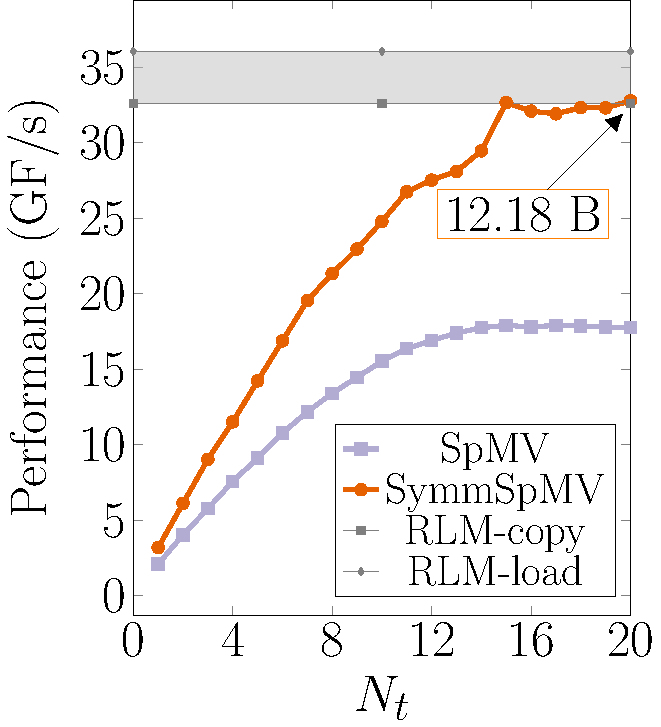
\includegraphics[width=0.23\textwidth , height=0.18\textheight]{pics/results/skx/corner_cases_scaling/plots/RCM/inline_1_RCM}}	
	\subfloat[\emph{parabolic\_fem}]{\label{fig:parabolic_fem_scaling}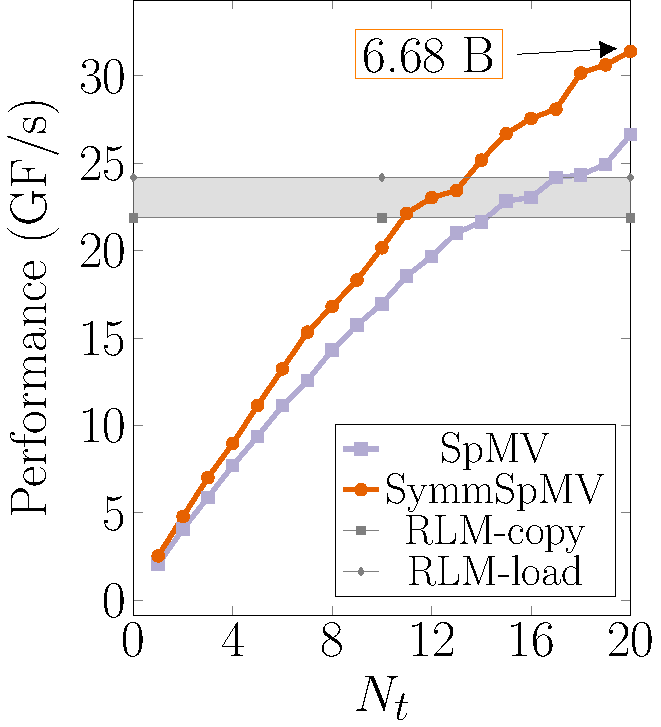
\includegraphics[width=0.23\textwidth , height=0.18\textheight]{pics/results/skx/corner_cases_scaling/plots/RCM/parabolic_fem_RCM}}
	\subfloat[\emph{Graphene-4096}]{\label{fig:Graphene-4096_scaling} 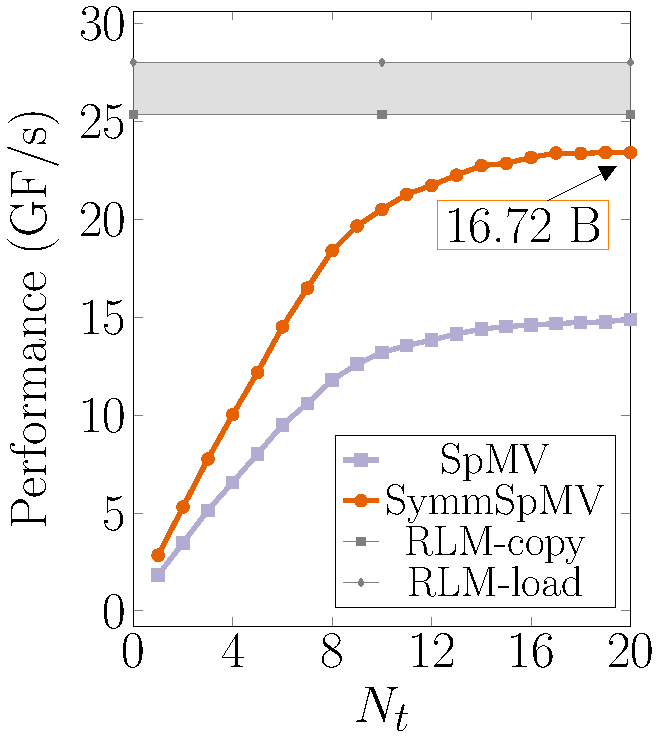
\includegraphics[width=0.23\textwidth , height=0.18\textheight]{pics/results/skx/corner_cases_scaling/plots/RCM/Graphene-4096_RCM}}	
	\caption{Parallel performance measurements of \acrshort{SymmSpMV}
	with \acrshort{RACE} on one \SKX socket for the four
	corner case matrices. The performance of the
	basic \acrshort{SpMV} kernel is presented for reference. For the
	matrices \Cref{fig:inline_scaling,fig:parabolic_fem_scaling,fig:Graphene-4096_scaling}
	the maximum \roofline performance limits \Cref{eq:upper_performance} are
	given using the computational intensity \Cref{eq:SymmSpMV_intensity} for
	the two extreme cases of load-only memory bandwidth (RLM-load) and copy
	memory bandwidth (RLM-copy). The measured full socket main memory data
	traffic per nonzero entry of the symmetric matrix (in \BYTE) for the \acrshort{SymmSpMV}
	 operation is also shown, where values below 12 \BYTE indicate caching of the matrix entries.}
	\label{fig:corner_cases_scaling}
\end{figure}

We have demonstrated that a simple choice for the only set of RACE input
parameters $\{\epsilon_s; s=0,1,\ldots\}$ can extract sufficient parallelism for
most matrices considered in this study. Moreover, the parallel efficiency as
calculated by RACE in combination with the \roofline performance model is a good
indication for scalability and maximum performance of the actual computations.

\begin{comment}
\subsection{Corner Cases}



\Cref{fig:corner_cases_scaling} shows the scaling performance of \acrshort{SymmSpMV} and \acrshort{SpMV} (baseline) kernel for corner case matrices on one socket of \SKX architecture. Chosen corner case matrices represent different aspects and bottlenecks that appear either due to \acrshort{RACE} method or because of hardware capabilities.

The \emph{crankseg\_1} matrix is the worst in terms of performance. It does not scale well due to it's limited parallelism obtained using the \acrshort{RACE} method. This property of \emph{crankseg\_1} is well evident directly after doing the theoretical estimate based on $\eta$ as  seen in \Cref{fig:crankseg_param}. One could further see that the actual scaling run of the kernel seen in \Cref{fig:crankseg_scaling} is exactly in tune with that of the theoretical result. Note that due to this bottleneck of parallelism we didn't achieve much benefit from using \acrshort{SymmSpMV} compared to \acrshort{SpMV}.

The \emph{inline\_1} matrix although being third lowest in terms of parallelism in the entire set of test matrices, but it still achieves a high efficiency ($\eta$ = 0.85) for 20 threads (see \Cref{fig:inline_param}), leading to good scaling as seen in \Cref{fig:inline_scaling}. The saturation in performance after 15 threads is due to the fact that we hit the memory bottleneck, similar saturation behavior can also be observed for \acrshort{SpMV} which is embarrassingly parallel. The saturation occurs at the maximum achievable performance on the given architecture which could easily be verified using the \roofline model \cite{Williams_roofline} and intensity equations (see \Cref{subsec:test_kernels}) as shown below:
\begin{align*}
	% P_\mathrm{max} =&  2 \fracUnit{FMA AVX-512 instruction}{cy*cores}  * 8 \fracUnit{FMA}{FMA AVX-512 instruction} \\
	% & * 2 \fracUnit{Flop}{FMA} * 2.4 \fracUnit{Gcy}{s} * 20 \unit{cores} = 1536  \fracUnit{GFlop}{s} \\	 
	I_\mathrm{\acrshort{SpMV}} &= \frac{2}{8+4+\frac{8+16}{73}} = 0.162 \fracUnit{Flop}{byte} \text{, assuming best case : $\alpha = \frac{1}{\acrshort{NNZR}}$}\\
	P_\mathrm{\acrshort{SpMV}} &= b_s*I_\mathrm{\acrshort{SpMV}}; \text{  for memory-bound case}\\
	P_\mathrm{\acrshort{SpMV}} &= 0.162\fracUnit{Flop}{Bytes}*115\fracUnit{GByte}{s} = 18.6 \fracUnit{GFlop}{s}\\
\end{align*}

As seen we achieve 17.8 GFlop/s which is close to the theoretical maximum of 18.6 GFlop/s for \acrshort{SpMV}. Similar derivation can be done for \acrshort{SymmSpMV} and one could see $P_\mathrm{\acrshort{SymmSpMV}}$= 34.5 GFlop/s, which is approximately twice that of \acrshort{SpMV} since $I_\mathrm{\acrshort{SymmSpMV}}$ is almost a factor two higher than $I_\mathrm{\acrshort{SpMV}}$ for matrix with moderate \acrshort{NNZR} (see \Cref{eq:SpMV_intensity,eq:SymmSpMV_intensity}). From \Cref{fig:inline_scaling} one can observe that at saturation we reach close to theoretical values. A cushioning effect due to memory bandwidth bottleneck is also evident from \Cref{fig:inline_scaling}, where we see that due to this saturation decrease in $\eta$ to a certain extent would not effect the socket level performance, it would just shift the knee of saturation towards right.

In the case of \emph{parabolic\_fem} matrix we theoretically have a good efficiency as seen from \Cref{fig:parabolic_fem_param}, but here we do not see any saturation in performance (see \Cref{fig:parabolic_fem_scaling}), even \acrshort{SpMV} does not have this saturation behavior. If one calculates the maximum  theoretical performance by \roofline model and assuming memory-boundedness as shown in previous example one would see that $P_\mathrm{\acrshort{SpMV}}$=15 GFlop/s and $P_\mathrm{\acrshort{SymmSpMV}}$=19 GFlop/s, but we achieve more than these values in actual runs 26.5 and 31.5 GFlop/s respectively. This is because the matrix is small enough ($\approx$ 46 MB for full matrix and $\approx$ 23 MB for symmetric storage) to just fit in caches (combined L2 and L3) of the \SKX architecture. Since the caches scales well on this architecture we don't observe the saturation behavior. It should be noted that in this case comparison between \acrshort{SpMV} and \acrshort{SymmSpMV} cannot be done directly since for \acrshort{SpMV} the total data is almost close to cache limits, while for \acrshort{SymmSpMV} it would easily fit in cache.

\emph{Graphene-4096} matrix on the other hand is a matrix with efficiency similar to \emph{parabolic\_fem} but with much larger size ($\approx 2 GB$) resulting in matrix data always coming from main memory. This therefore shows dominant saturation behavior and since we achieve good efficiency ($\eta$) the knee of saturation begins at a well early stage for \acrshort{SymmSpMV} compared to  the case of \emph{inline\_1} where the efficiency was lower in comparison resulting in smaller \acrshort{threadEff}.

\end{comment}

\begin{comment}
Quantifying quality of the method in a well-defined way is a primary and most vital step for parameter study. We do this using the concept of \effPar. From \Cref{Sec:race} we saw that even though one tries to achieve parallelism exactly as that required by the hardware, in practice one might not be able to utilize this parallelism to 100 \% due to load imbalances. Therefore we use a simple calculation based on the \levelTree to determine efficiency. This takes into account load imbalances incurred from different stages of recursion. We first calculate \effRow for each of the worker leaves (leaves in finest level) in \levelTree.
The \levelGroups (leaves) in \levelTree that are not further refined form worker leaves and they are responsible for executing the rows (nodes) in their range, the work done by these leaves is therefore directly proportional to the number of rows. Hence the \effRow of these worker leaves is same as number of rows (\acrshort{nrows}), for example in case of $T_0(0)$ \effRow ( $\acrshort{nrowsEff}(T_0(0))$ = $\acrshort{nrows}(T_0(0))$ ) is 14 and $\acrshort{nrowsEff}(T_1(0) \subset T_0(4))$ is 6. After calculating the \effRow for worker leaves the information is propagated to other leaves in lower stages (up in the \levelTree) as follows: 
\begin{align*}
\acrshort{nrowsEff}(T_s(i)) &= \max\left(\acrshort{nrowsEff}(T_{s+1}(j) \subset T_s(i))\right) + \max\left(\acrshort{nrowsEff}(T_{s+1}(k) \subset T_s(i))\right)\\
 & \text{for } j \text{ is even and } k \text{ is odd}
\end{align*}

Such a definition for \effRow is based on the idea that a parent has to wait until the child leaf with most number of rows in each sweep (color) has finished it's work due to synchronization needed with it's siblings. This has to be handled separately for each of the two parallel sweep (colors) as there is this synchronization happening after each of the sweeps (colors). 

Once the information is propagated up the tree and as it reaches the root we have a single \effRow ($\acrshort{nrowsEff}(T_{-1})$) for the entire tree, which has taken into account load imbalance happening between all \levelGroups in all stages. The ratio of total number of rows ($\acrshort{nrows}^{total}$) in the entire matrix to that of $\acrshort{nrowsEff}(T_{-1})$ gives \effPar, denoted as \acrshort{threadEff}. Efficiency ($\eta$) of the method is then defined as ratio of  \acrshort{threadEff} to that of required hardware parallelism (\acrshort{nthreads}). 

\begin{align}
	\acrshort{threadEff} &= \frac{\acrshort{nrows}^{total}}{\acrshort{nrowsEff}(T_{-1})} \\
	\eta &= \frac{\acrshort{threadEff}}{\acrshort{nthreads}} \label{eq:eta}
\end{align}

For example in our \stex, \Cref{fig:rec_2d-7pt_tree} shows \acrshort{nrowsEff} for each leaves in angular brackets and here $\acrshort{threadEff} = 5.8$ and $\eta = 0.725$. The value of $\eta = 1$ implies there is perfect load balancing which is almost impossible. In general $0 < \eta \leq 1$. This parameter $\eta$ will be used as a measure of quality in parameter study.

\subsection{Case study}
A given matrix has a fixed amount of parallelism and as the amount of required parallelism (\acrshort{nthreads}) increases load balancing degrades due to more threads per stage and imbalances between stages. The rate of degradation can however be controlled to certain extent by the tolerance $\epsilon_s$ (see \Cref{eq:epsilon}) specified while choosing a \levelGroup. Typical value of $\epsilon_s$ is in range of [0.4,0.9]. Having a small $\epsilon_s$ (for example 0.4) implies we utilize the current stage `s' to maximum and do not impose high load balancing constraint, a high value on the other hand requires more balanced load from current stage `s'. 

Test matrices (see \Cref{Sec:test_bed}) considered have a varying degree of parallelism, and in order to see the effect of $\eta$ and $\epsilon_s$ we choose the \emph{inline} matrix. The choice is due to the fact that this matrix has relatively small amount of parallelism and this allows us to demonstrate various effect, ranging from good to bad case scenario with small number of parallelism (\acrshort{nthreads}$ < 200$). This limited parallelism can be observed from \Cref{fig:inline-a} 
where efficiency keeps on decreasing with \acrshort{nthreads} for \emph{inline} matrix. Similar behavior can be observed for \emph{crankseg\_1}, \emph{F1} and \emph{ship} matrices, of which \emph{crankseg\_1} being the worst. For majority of other test matrices one could observe that efficiency $\eta$ initially drops but then remains almost constant in the range $\eta$ = [0.50,0.80] (depending on matrix) for the entire scanned area of $1 \leq $\acrshort{nthreads}$ \leq 200$.

%\begin{figure}[tbhp]
%	\centering
%	\subfloat[$\eta$ vs \acrshort{nthreads} for \emph{inline} matrix ]{\label{fig:inline-a}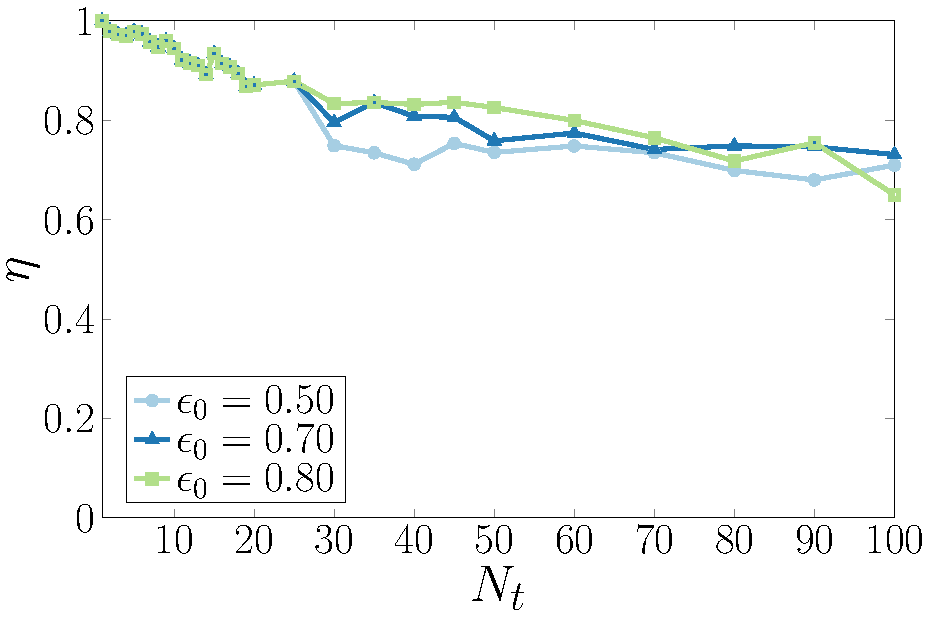
\includegraphics[width=0.45\textwidth , height=0.2\textheight]{pics/param_study/threads_vs_eff}}
%	\hspace{1.5em}
%	\subfloat[Effect of $\epsilon_0$ at low \acrshort{nthreads}, \acrshort{nthreads}=25]{\label{fig:inline-b}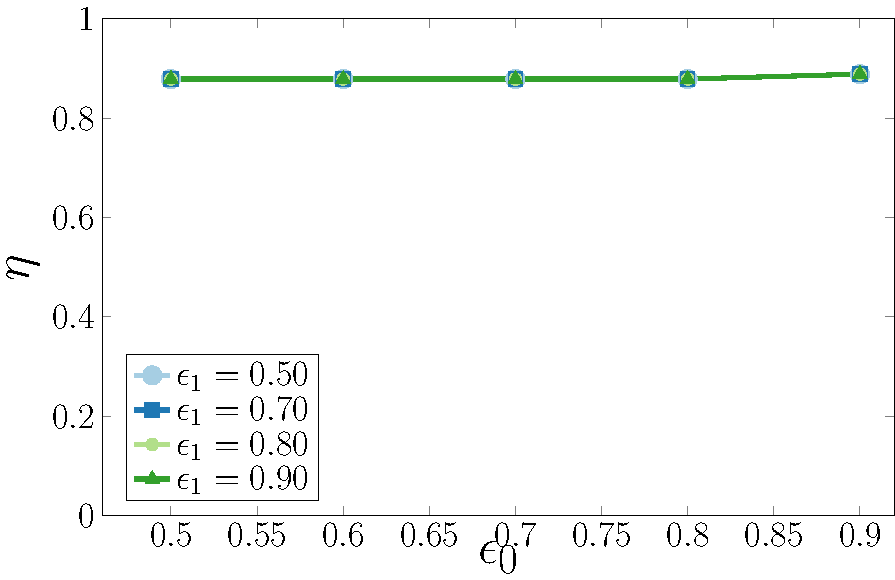
\includegraphics[width=0.45\textwidth , height=0.2\textheight]{pics/param_study/scaling_eps_1_25_threads}}
%	
%	\subfloat[Optimal $\epsilon_0$ lowered and optimal $\epsilon_1$ = 0.9, \acrshort{nthreads}=45 ]{\label{fig:inline-c}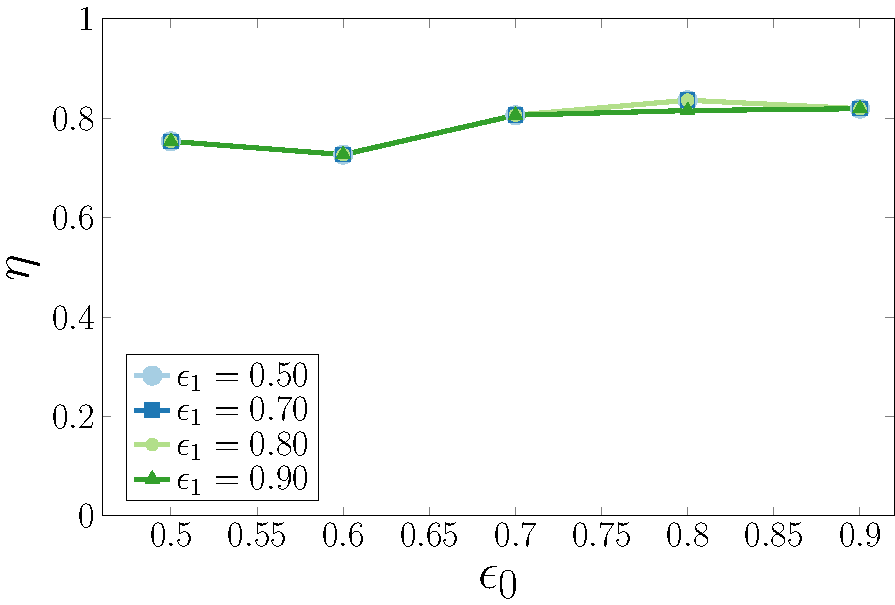
\includegraphics[width=0.45\textwidth , height=0.2\textheight]{pics/param_study/scaling_eps_1_45_threads}}
%	\hspace{1.5em}
%	\subfloat[Optimal $\epsilon_0$ lowered to 0.4 and $\epsilon_1$ to 0.7, \acrshort{nthreads}=100 ]{\label{fig:inline-d}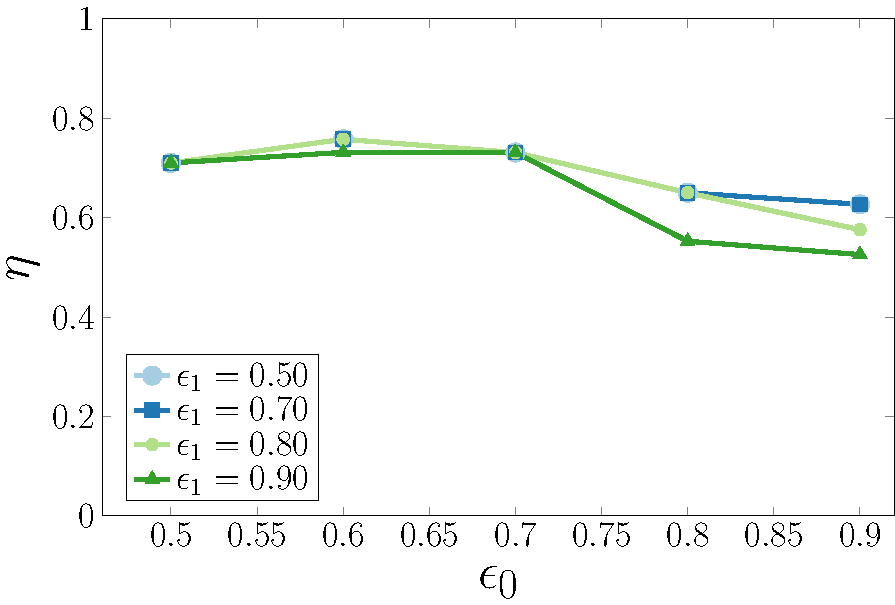
\includegraphics[width=0.45\textwidth , height=0.2\textheight]{pics/param_study/scaling_eps_1_100_threads}}
%	\caption{Parameter study on \emph{inline} matrix. In \Cref{fig:inline-b,fig:inline-c,fig:inline-d} each lines in the plot are iso-$\epsilon_2$ and impact of $\eta$ with respect to $\epsilon_1$ is shown.}
%	\label{fig:inline_param_study}
%\end{figure}

At small number of threads (\acrshort{nthreads}) all matrices have high efficiency (like $\eta>0.8$). As there is a lot of parallelism in this stage compared to requirement, $\eta$ is insensitive of $\epsilon_s$. The value of \acrshort{nthreads} upto which such a behavior can be observed varies from matrix to matrix, for example \emph{inline} shows this upto \acrshort{nthreads}$\approx20$, while for matrix like \emph{Graphene} this is grater than $200$.  Further increasing \acrshort{nthreads} one could observe $\eta$ starts to vary with $\epsilon_0$. For example in case of \acrshort{nthreads}$ = 25$ one could see in \Cref{fig:inline-b} maximum $\eta$ is achieved with high value of $\epsilon_0$ (0.9) due to good load balancing. But as 
\acrshort{nthreads} further increase the optimal $\epsilon_0$ starts shifting towards left (see \Cref{fig:inline-c}),
 since one requires more parallelism from the current stage (s=0) and higher $\epsilon_0$ would be decremental since it would require the \levelTree to go more deep and hence load imbalances in next stages will get multiplied. $\epsilon_1$ which till now didn't effect much starts to influence slowly as \acrshort{nthreads} increments again, for example in case of \emph{inline} till $\acrshort{nthreads}=90$ $\epsilon_1=0.9$ was optimal, but then the optimal $\epsilon_1$ reduces and reaches $0.7$ at \acrshort{nthreads}$=190$ as seen in \Cref{fig:inline-d}. $\eta$ would start to get affected by $\epsilon_s$ of next stages in similar manner with increase of \acrshort{nthreads}.
 
Behavior of other matrices in the test bed follow similar pattern, but \acrshort{nthreads} at which different phases occur varies from matrix to matrix.  \Cref{fig:param_all_mtx_stat} gives a broad overview of the efficiency ($\eta$) behavior of entire test matrices using scatter plot. Each point at a specific \acrshort{nthreads} represents efficiency ($\eta$) of a matrix. Majority of test matrices having an initial drop in $\eta$ and then remaining constant is reflected in the statistical plot. The lowest points in the plot correspond to \emph{crankseg\_1} matrix, here we achieve only a mere parallelism of eight at maximum (\acrshort{threadEff} = 8), while the upper points correspond to matrix having highest parallelism namely \emph{Graphene} matrix.

In practice for a given matrix it's difficult to precisely determine the optimal rate of decrease in $\epsilon_s$ without parameter search, and therefore selecting proper $\epsilon_s$ for given \acrshort{nthreads} can be challenging. One idea is to see total levels (\acrshort{totalLvl}) and distribution of nonzeros (\acrshort{nnz}) in different levels of current stage `s' and heuristically determine $\epsilon_s$ based on the pressure of parallelism from stage `s'. This is not currently done and is part of our future work. As a rule of thump an $\epsilon_{0,1} = 0.8$ and $\epsilon_{s>1} = 0.4$ is sufficient for most matrices on current architectures, therefore currently for experiments we set these $\epsilon_s$ values for all matrices.

 In \Cref{fig:corner_cases_param} we have plotted \acrshort{threadEff} and $\eta$ vs \acrshort{nthreads} for corner case matrices with the settings used in experiment runs. Here we set $\epsilon_{0,1}=0.8$ and use \acrfull{RCM} in the \emph{level construction} stage (\Cref{subsec:LEVEL_CONST}). Big fluctuation in \emph{crankseg\_1} is due to the fact that we set high load balancing requirement (high $\epsilon_s$ factor) and as seen in the example of \emph{inline\_1} matrix this is not optimal when we reach the limit of parallelism. The theoretical estimates obtained in \Cref{fig:corner_cases_param} will be directly used to compare with experiment runs in the next section (\Cref{Sec:expt}).

\end{comment}
